% !TeX root = ../main.tex
% Add the above to each chapter to make compiling the PDF easier in some editors.
%------------------------------------------------------------------------
\chapter{Tuning Linear Programming Solvers for Query Optimization}\label{chapter:linearprogramming}

%------------------------------------------------------------------------
%------------------------------------------------------------------------
\section{Proposal or Implementation}
Our contribution consists in conducting experiments on small packing LP problems that are generated from
real-life queries as mentioned in Section \ref{section:cardinality-estimate} as well as randomly generated
LPs with varying sizes. We use different LP solvers, and different update methods to solve these LPs.
We then proceed to compare results based on time and memory performance. We also build an analysis of our datasets' properties.
Finally, we aim to give a recommendation on how to build the best performing LP solver based on the
particularities of the LP problems.

%------------------------------------------------------------------------
\subsection{Implementation hierarchy}
The final code repository contains 3 different solvers as shown in the
UML graph \ref{fig:hierarchy}
and a \verb|compareSolvers.cpp|, in which we can conduct our benchmarks.
\begin{figure}[htpb]
    \centering
    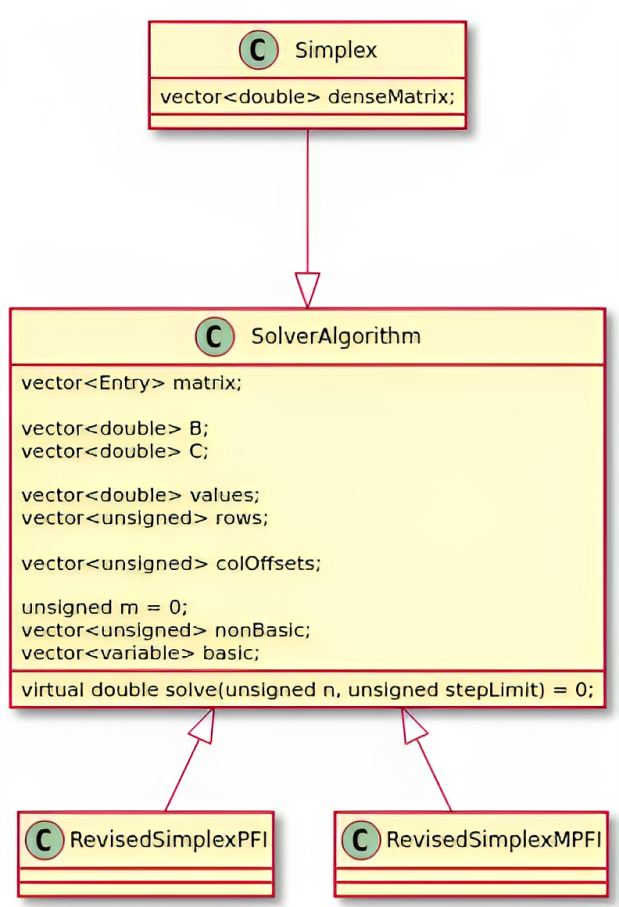
\includegraphics[height=0.6\textheight]{figures/UML.png}
    \caption{An UML Graph explaining the hierarchy of the implementation}
    \label{fig:hierarchy}
\end{figure}

%------------------------------------------------------------------------
\subsection{Tableau simplex solver}
This solver is the simplest of the three solvers, it follows the steps of the standard simplex
algorithm in its tabular form. It uses dense matrices and vectors. Although the
doPivotting() is costly, the simplicity of this algorithm makes it suitable for
smaller problems.
\begin{algorithm}
    \caption{Tableau Simplex Algorithm}
    \begin{algorithmic}[1]
        \State \textbf{Input:} Packing LP maximisation problem in computational form
        \State \textbf{Output:} Optimal value $z$

        \State \textbf{Step 1:} Pricing: Find pivot column, or entering variable using Bland's rule
        \State \hspace{\algorithmicindent} $enteringVars \gets \text{findPivotColumnCandidates}()$
        \State \hspace{\algorithmicindent} \textbf{if} no entering variable found \textbf{then}
        \State \hspace{\algorithmicindent} \hspace{\algorithmicindent} \text{print} "Optimal value reached."
        \State \hspace{\algorithmicindent} \hspace{\algorithmicindent} \Return $z$
        \State \hspace{\algorithmicindent} \textbf{end if}
        \State \hspace{\algorithmicindent} $pivotColumn \gets enteringVars[0]$

        \State \textbf{Step 2:} Find pivot row, or leaving variable using the ratio test
        \State \hspace{\algorithmicindent} $pivotRow \gets \text{findPivotRow}(pivotColumn)$
        \State \hspace{\algorithmicindent} \textbf{if} no leaving variable \textbf{then}
        \State \hspace{\algorithmicindent} \hspace{\algorithmicindent} \text{print} "The given LP is unbounded."
        \State \hspace{\algorithmicindent} \hspace{\algorithmicindent} \Return $\infty$
        \State \hspace{\algorithmicindent} \textbf{end if}

        \State \textbf{Step 3:} Update the tableau using pivotting and update the objective function value
        \State \hspace{\algorithmicindent} $\text{doPivotting}(pivotRow, pivotColumn, z)$

        \State \textbf{Goto Step 1}
    \end{algorithmic}
\end{algorithm}
%------------------------------------------------------------------------
\subsection{Data structures}

\subsubsection{Dense Matrix}
Given a matrix \( A \) of dimensions \( m \times n \), the density \( D \) of
the matrix is defined as:
\[
    D(A) = \frac{\text{Number of non-zero elements in } A}{m \times n}
\]
$D$ is a measure between 0 and 1, where 0 indicates a
matrix with all zero elements (completely sparse)
and 1 indicates a matrix with all non-zero elements (completely dense).
Sparsity of a matrix is a feature that can be exploited to
enhance memory complexity of our implementation, as we will discuss next.

\subsubsection{Sparse Matrix}\label{subsubsection:sparse-matrix}
In our dataset, we deal with sparse matrices.
We use the \gls{ccr} format to store sparse matrices in C++. They are represented using this
structure.

\begin{verbatim}
      struct CCRMatrix {
          float *values;  // Non-zero values in the matrix
          int *rowIdx;  // Row indices corresponding to the non-zero values
          int *colPtr;  // Points to the index in `values` where each column starts
      };
\end{verbatim}

For example, consider the matrix \( A \):
\[
    A =
    \begin{bmatrix}
        5 & 0 & 0 \\
        0 & 8 & 0 \\
        0 & 0 & 3 \\
        0 & 6 & 0 \\
    \end{bmatrix}
\]

In \gls{ccr} format, the matrix is represented using three arrays:
\texttt{values}, \texttt{row\_indices}, and \texttt{column\_pointers}.

\begin{align*}
    \texttt{values}           & = [5, 8, 6, 3] \\
    \texttt{row\_indices}     & = [0, 1, 3, 2] \\
    \texttt{column\_pointers} & = [0, 1, 3, 4] \\
\end{align*}
\subsubsection{Comparison of memory complexity}
Storing a dense matrix variable \( A \) of dimensions \( m \times n \) in C++, we have two alternatives.
\begin{itemize}
    \item using an array of arrays (two-dimensional array) or \texttt{vector<vector<double>>}. This array would contain
          $m$ arrays, representing the rows, each contains $n$ doubles, representing the matrix entries in each row.
    \item using a one-dimensional array with rows stacked next to each other,
          \texttt{vector<vector<double>>}. This array contains $m \times n$ entries.
          With the $a_{row,col}$ entry located at \texttt{A[row * (m + n) + col]}
\end{itemize}
Note that even
though there is a difference between  \texttt{array}, \texttt{vector} and \texttt{list}, we
choose \texttt{std::vector}, or dynamoic array, in all our implementation, because it suits our purpouses.
We also opt for 1D array as opposed to 2D array for better memory complexity and speed.
We explain this choice:
The 2D array typically requires slightly more memory than its 1D counterpart.
This increased memory usage is attributed to the pointers in the 2D array that point to
the set of allocated 1D arrays. While this difference might seem negligible for large arrays,
it becomes relatively significant for smaller arrays. In terms of speed, the 1D array often outperforms
the 2D array due to its contiguous memory allocation, which reduces cache misses.
However, the 2D dynamic array loses cache locality and consumes more memory because of its non-contiguous
memory allocation. While the 2D dynamic array introduces an
extra level of indirection, the 1D array has its own overhead stemming from index calculations.

\begin{figure}[h]
    \centering
    \caption{Memory Layout of a 1D Dynamic Array}
    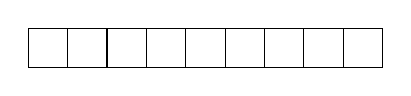
\begin{tikzpicture}[scale=0.5, every node/.style={scale=0.5}]
        \foreach \x in {0,...,8} {
                \draw (\x,0) rectangle ++(1,1);
            }
    \end{tikzpicture}
\end{figure}

\begin{figure}[h]
    \centering
    \caption{Memory Layout of a 2D Dynamic Array}
    \begin{tikzpicture}[scale=0.5, every node/.style={scale=0.5}]
        \foreach \x in {0,...,2} {
                \draw (\x,2) rectangle ++(1,1);
            }
        \foreach \x in {0,...,2} {
                \foreach \y in {0,...,2} {
                        \draw (\x*4+\y,-\x) rectangle ++(1,1);
                    }
            }
        \draw[->] (0.5,2) -- (0.5,1);
        \draw[->] (1.5,2) -- (1.5,1.25) -- (4.5,1.25) -- (4.5,0);
        \draw[->] (2.5,2) -- (2.5,1.5) -- (8.5,1.5) -- (8.5,-1);
    \end{tikzpicture}
\end{figure}


%------------------------------------------------------------------------
\subsection{Revised Simplex Solver}


%------------------------------------------------------------------------
\subsection{Stability}
Mention zero tolerances: A zero tolerance epsilon2 saefguards against divisions
by extremely small numbers, which tend to produce the most dangerous rounding errors, and
may even lead to degeneracy. diagonal entry in eta matrix should be fairly far from
otherwise (in our experiment) degeneracy.

%------------------------------------------------------------------------

%------------------------------------------------------------------------
\section{Experiments and Results}
All the following results have been obtained on a system with the following settings:
\begin{itemize}
    \item OS: Ubuntu 22.04.1 LTS x86\_64
    \item Host: 82A2 Yoga Slim 7 14ARE05
    \item CPU: AMD Ryzen 7 4800U with Radeon Graphics (16) @ 1.800GHz
    \item GPU: AMD ATI 03:00.0 Renoir
    \item RAM: 10409MiB / 15363MiB
\end{itemize}

Presolve techniques are not used, the solvers assume an input of the form explained
in the UML graph \ref{fig:hierarchy} and in the format input as described
in the following section.

The computed optimal solutions have been validated using the scipy python library,
our solvers terminate and deliver correct optimum.

\subsubsection{Note on cache locality}
Through our experiments, we have noticed that if we call our C++ solvers
consecutively, this may affect the recorded exectuin times and thus make our benchmarks
unreliable or inaccurate. This may be due to cache locality: If the second solver is working
on data that was recently processed by the first solver, it might benefit from cache locality,
as some of the required data
might still be in the cache. This can lead to faster execution times for the second solver.
However, if the first solver used a significant amount of memory and displaced data relevant
to the second solver from the cache, then the second solver might experience cache misses.
Cache misses
can slow down the execution as the CPU has to fetch the required data from the main memory.
We detect varying results when we switch the order in which we call our solvers, and so
this effect is likely significant.
Our solution to avoid this is by isolating the solvers, and calling each one independently
(by commenting out any calls to the others). This is our approach to receive
accurate performance measures, and be able to compare the solvers reliably.

%------------------------------------------------------------------------
\subsection{Query datasets}
The input files \texttt{TPCH}, \texttt{TPCDS}, and \texttt{JOB} contain packing
\gls{lp} problems. We have already established the mathematical derivation of how
these query-related packing
\gls{lp} problems are generated in \ref{section:cardinality-estimate}.

The \texttt{lp.txt} file is structured for machine readability.
In this format, each line represents a single \gls{lp}. The line starts with
the number of rules in that problem. For each rule, the number of entries in
the coefficient matrix is specified first, followed by pairs of values:
the column number and the coefficient. This is convenient to parse the entries
and then populate our sparse matrix representation quite efficiently.

\begin{lstlisting}
lp:
8 2 0 0.0540277 2 0.0540277 ...
\end{lstlisting} \label{format_input}

\begin{table}[!htb]
    \centering
    \caption{Benchmarks and number of queries.}
    \begin{tabular}{|l|l|}
        \hline
        Benchmark                                & Number of Queries \\
        \hline
        JOB \parencite{10.14778/2850583.2850594} & 2230              \\
        TPC-H \parencite{tpch}                   & 16                \\
        TPC-DS \parencite{tpcds2022}             & 148               \\
        \hline
    \end{tabular}
    \label{job_tpch_tpcds}
\end{table}

\subsubsection{The JOB dataset results}
In the table \ref{table_job_stats} are some important statistical finds following our
experiments with the JOB dataset.
This is the largest dataset of all three query datasets. It contains duplicated queries so we
perform a removal of the duplicated LPs before. We collect the data and perform plotting and data summary
using R scripts.

\begin{figure}[!htb]
    \centering
    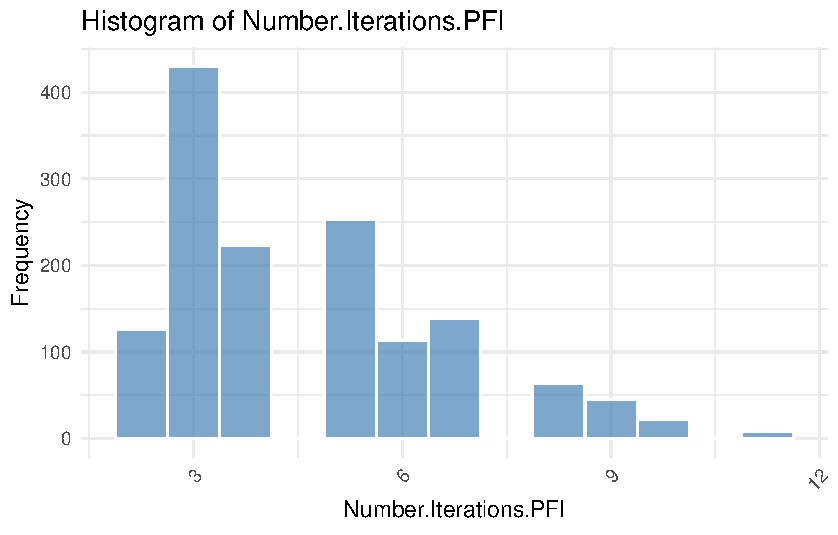
\includegraphics[width=\textwidth]{figures/histo_iter_pfi.pdf}
    \caption{Boxplot for number of iterations for PFI for JOB dataset}
    \label{fig:num_iter_boxplot_pfi_job}
\end{figure}

\begin{figure}[!htb]
    \centering
    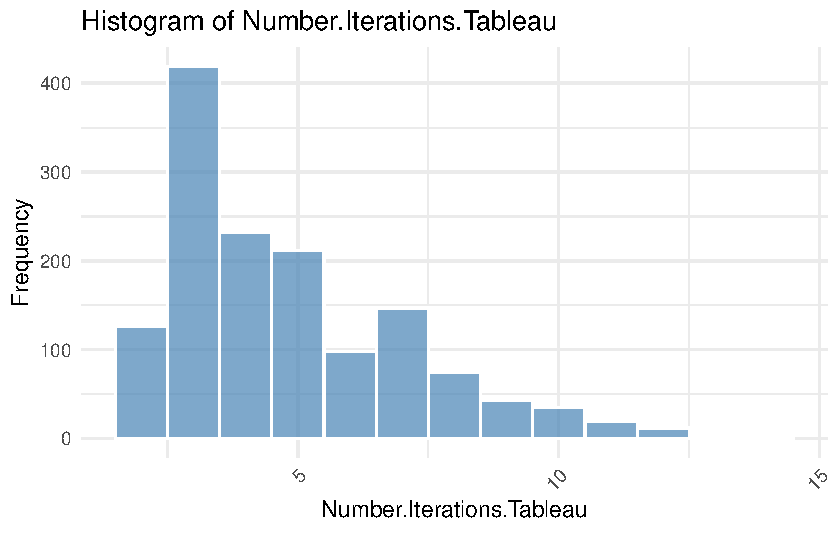
\includegraphics[width=\textwidth]{figures/histogram_iter_tableau.pdf}
    \caption{Boxplot for number of iterations for Tableau for JOB dataset}
    \label{fig:num_iter_boxplot_tableau_job}
\end{figure}


\begin{figure}[!htb]
    \centering
    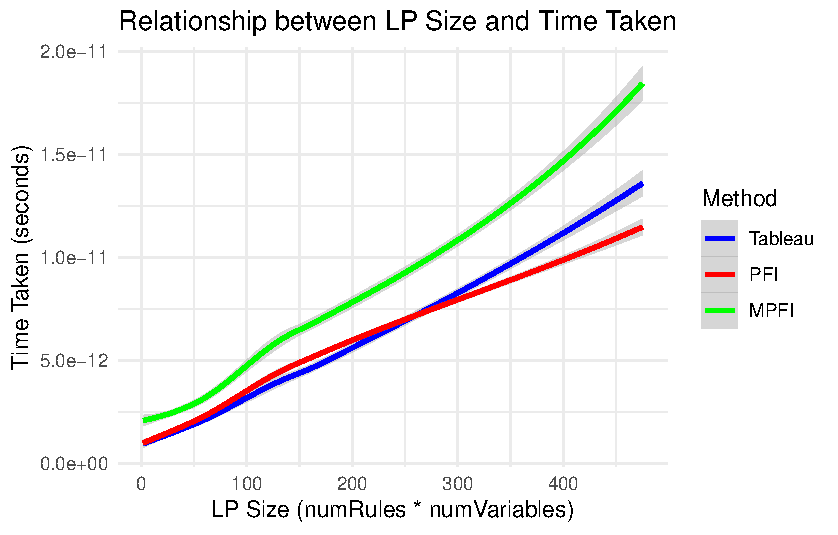
\includegraphics[width=\textwidth]{figures/lp_size_vs_time_job.pdf}
    \caption{Relation between LP size and time for the 3 simplex solvers for JOB dataset.}
    \label{fig:lp_size_vs_time_job}
\end{figure}

\begin{table}[!htb]
    \centering
    \caption{Statistics about JOB dataset}
    \begin{tabular}{lrrrr}
        \toprule
        Variable                  & Min    & Median  & Mean    & Max     \\
        \midrule
        LP size                   & 2.00   & 54.00   & 94.56   & 475.00  \\
        Number of Rules           & 1.000  & 6.000   & 7.037   & 19.000  \\
        Number of Variables       & 1.00   & 3.00    & 3.07    & 6.00    \\
        Constraint Matrix Density & 0.3684 & 0.6667  & 0.6703  & 1.0000  \\
        Solution Time Scipy       & 650    & 931     & 959     & 1802    \\
        Solution Time Cplex       & 97.04  & 184.06  & 190.66  & 415.56  \\
        Solution Time Tableau     & 2.00   & 4.00    & 12.15   & 4274.00 \\
        Solution Time PFI         & 2.000  & 6.000   & 8.316   & 65.000  \\
        Solution Time MPFI        & 1.000  & 4.000   & 5.517   & 68.000  \\
        Number Iterations Tableau & 2.000  & 4.000   & 4.829   & 14.000  \\
        Number Iterations PFI     & 2.000  & 4.000   & 4.621   & 11.000  \\
        Number Iterations MPFI    & 2.000  & 4.000   & 4.671   & 13.000  \\
        Optimal Value             & 0.3188 & 20.6702 & 21.8575 & 42.1804 \\
        \bottomrule
    \end{tabular}
    \label{table_job_stats}
\end{table} 

This is our results:
\begin{table}[!htb]
    \centering
    \caption{Number of LPs or Queries Solved by Hour for the JOB dataset}
    \begin{tabular}{l|r}
        \toprule
        Method                     & Number of LPs/Queries \\
        \midrule
        Revised Simplex MPFU Umbra & 906,607,929           \\
        Tableau Simplex            & 1,400,923,787         \\
        Revised Simplex PFI        & 1,287,140,216         \\
        Scipy (method highs)       & 4,069,108             \\
        Cplex                      & 17,849,851            \\
        \bottomrule
    \end{tabular}
    \label{table_lps_hr_job}
\end{table} 


\begin{figure}[p]
    \begin{adjustbox}{width=\paperwidth,center}
        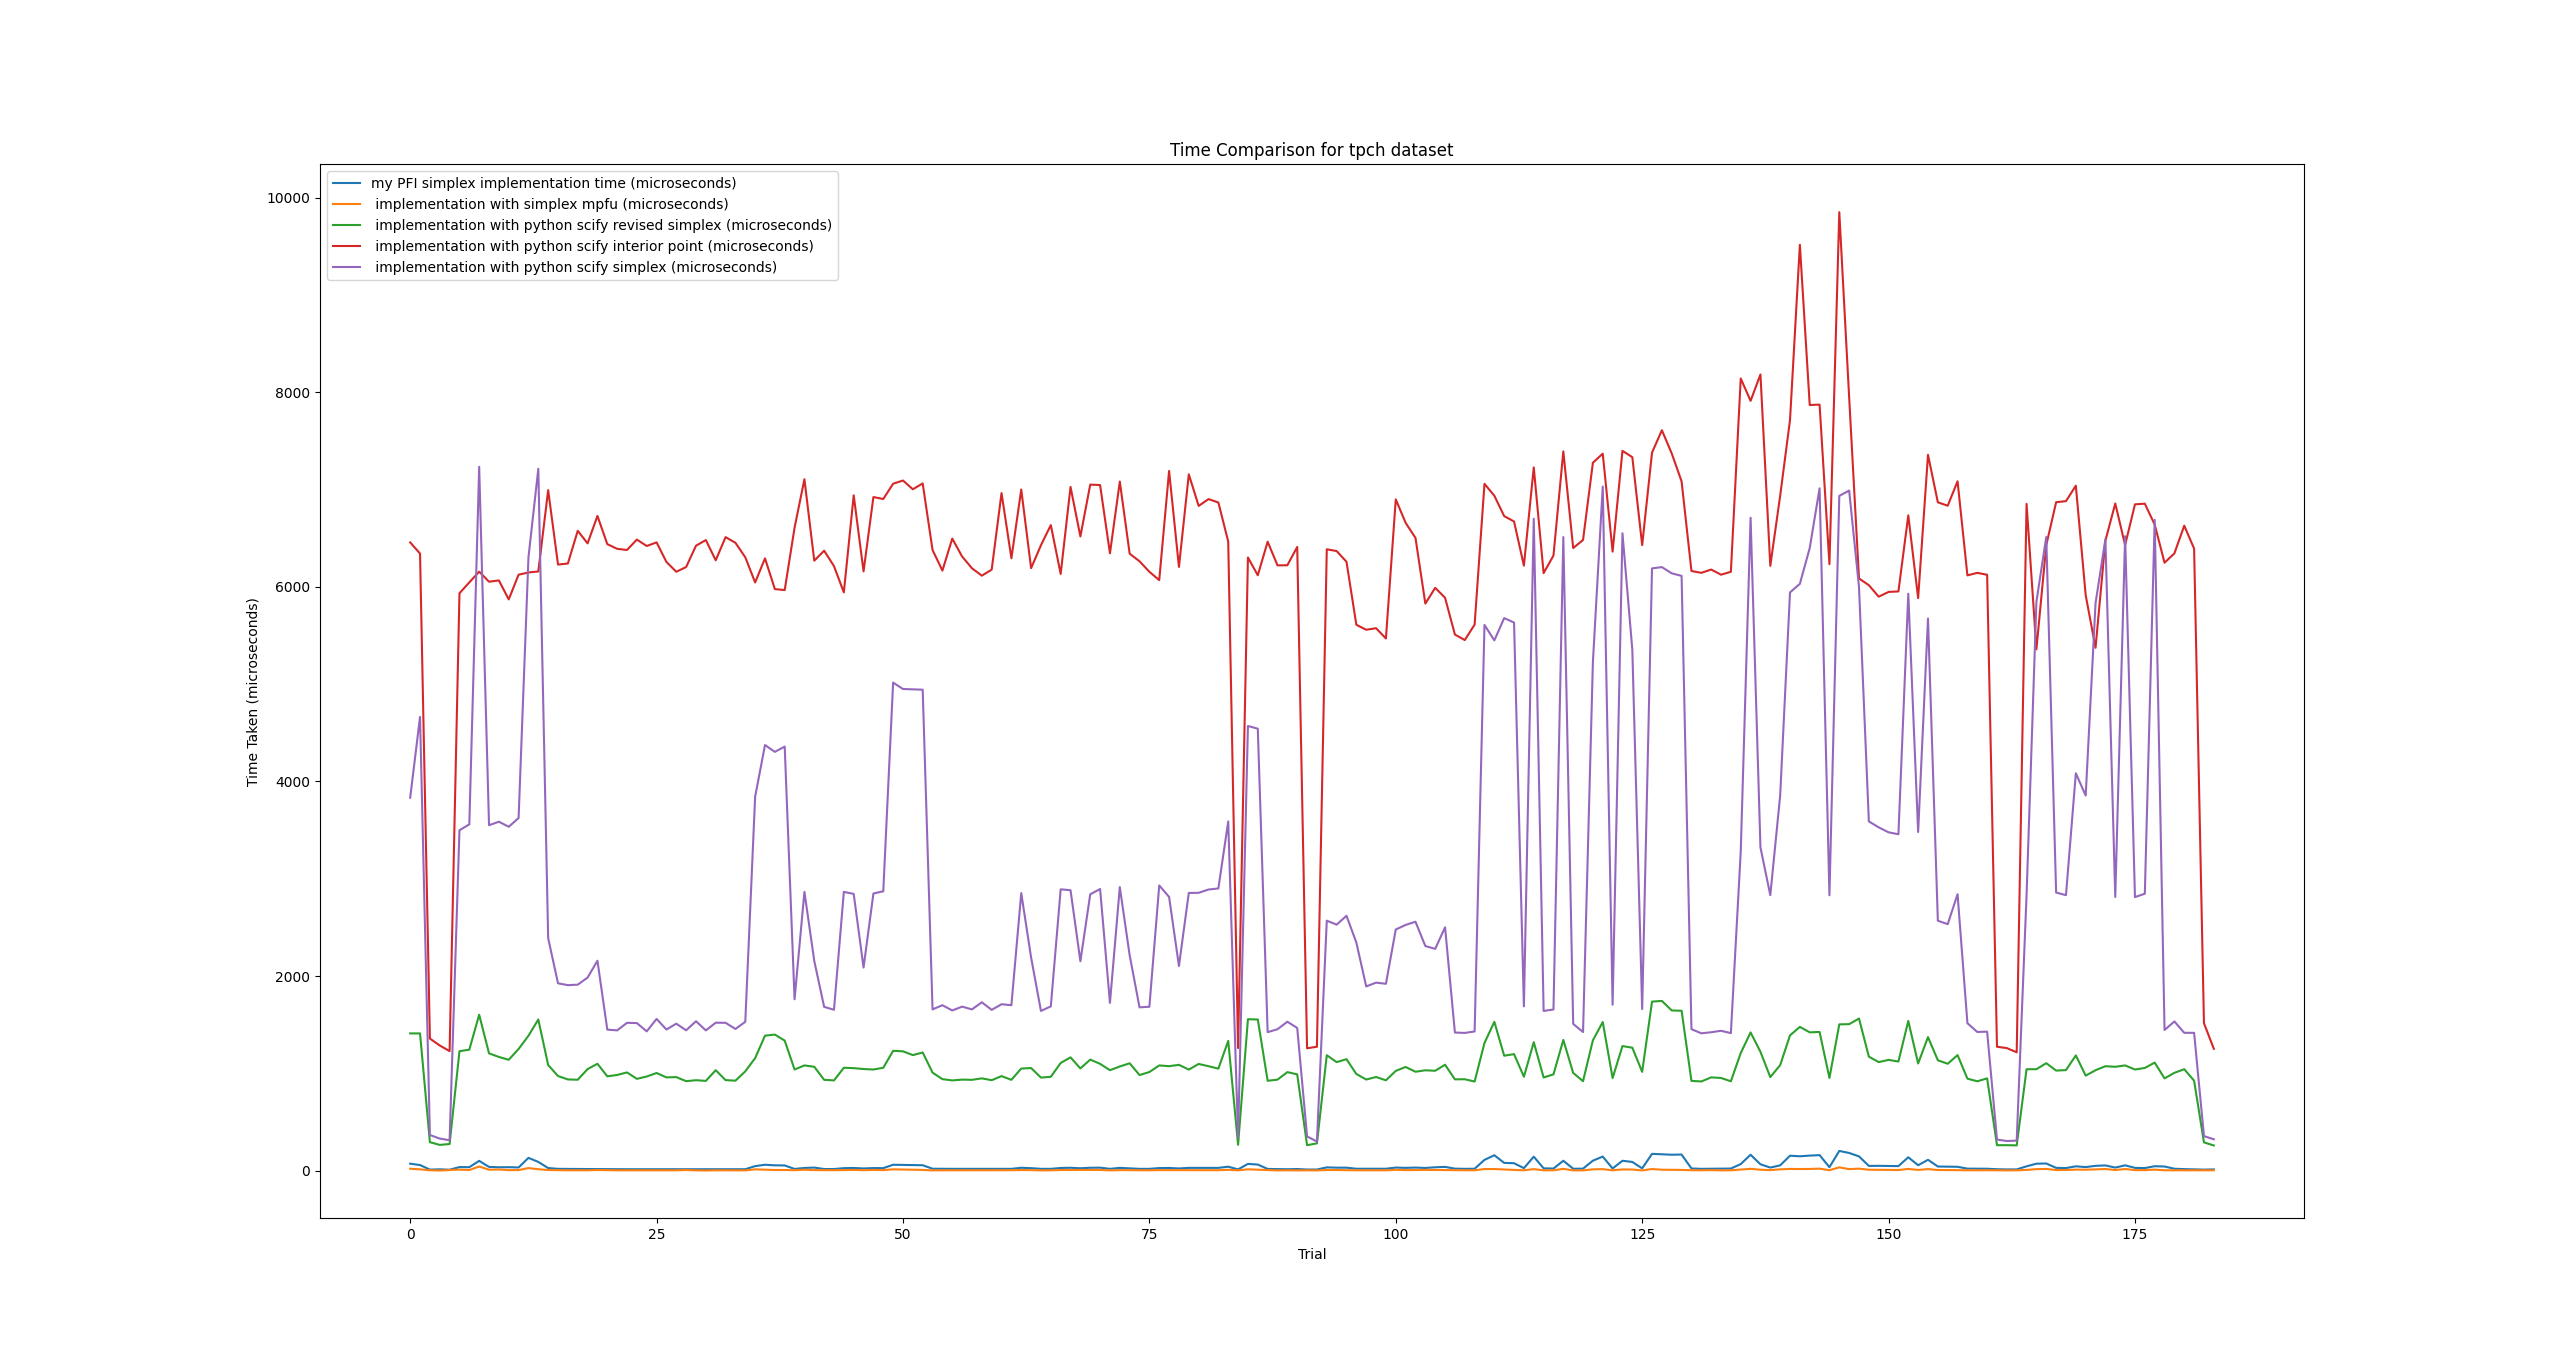
\includegraphics[width=\paperwidth]{figures/all_scify_mpfi_pfi.png}
    \end{adjustbox}
    \caption{A graph comparing the time performance of two of
        our solvers with scipy solver solving the tpch dataset}
    \label{fig:all_time_tpch}
\end{figure}



\subsubsection{TPC-DS results}

\begin{figure}[!htb]
    \centering
    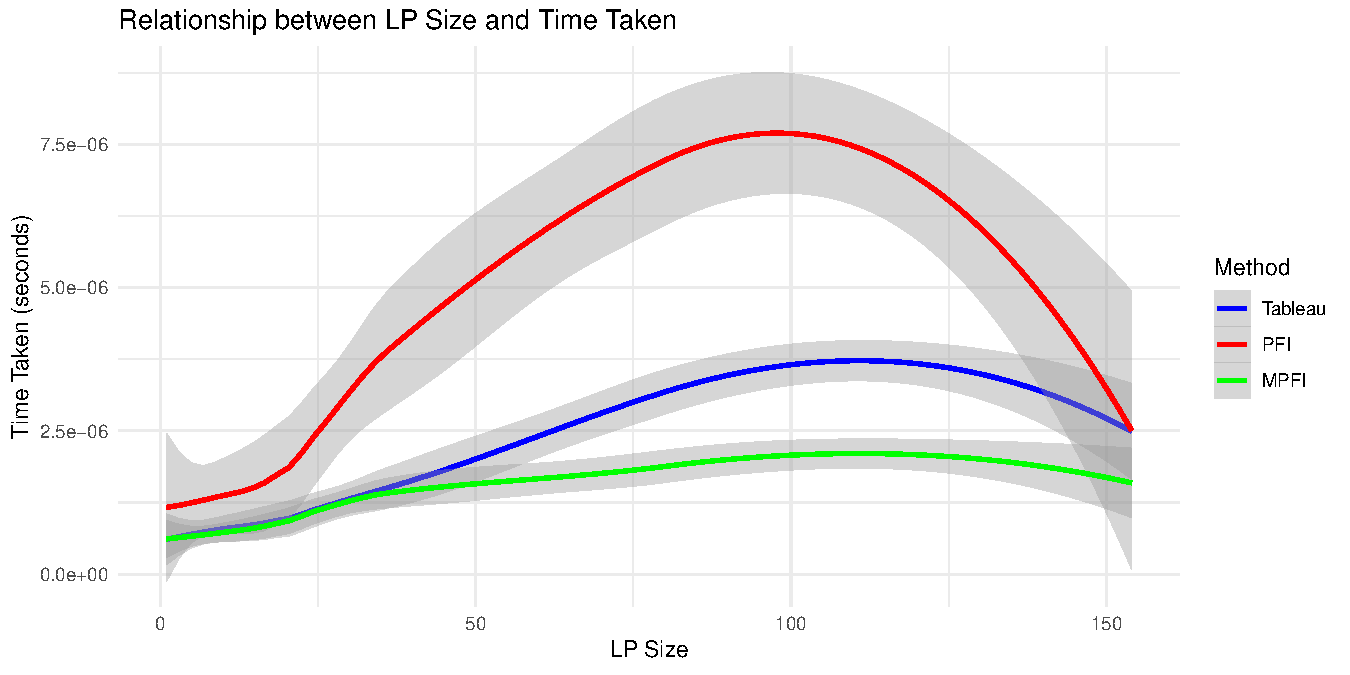
\includegraphics[width=\linewidth]{figures/methods_time_tpcds.pdf}
    \caption{A graph comparing the time performance of two of
    our solvers with scipy solver solving the tpcds dataset}
    \label{fig:methods_time_tpcds}
\end{figure}

\begin{figure}[!htb]
    \centering
    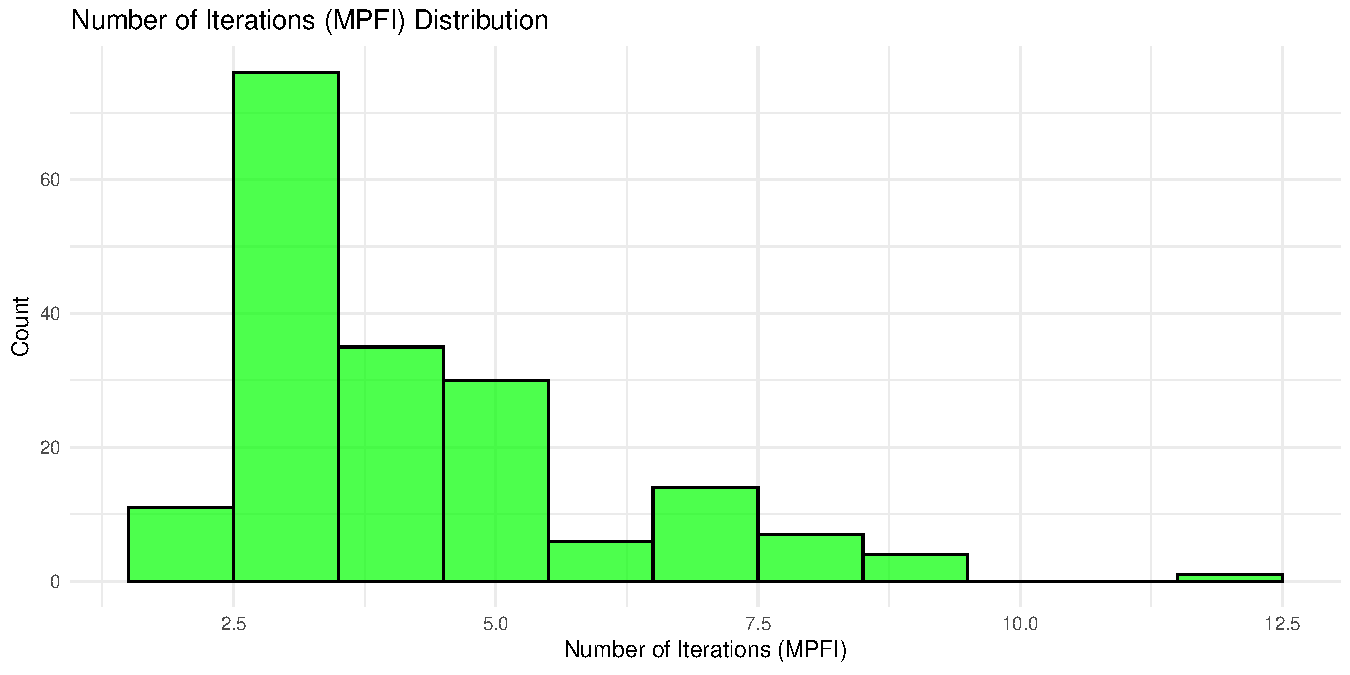
\includegraphics[width=\linewidth]{figures/num_iter_tpcds_mpfi.pdf}
    \caption{Boxplot for number of iterations for MPFI for TPCDS dataset}
    \label{fig:num_iter_tpcds_mpfi}
\end{figure}

\begin{figure}[!htb]
    \centering
    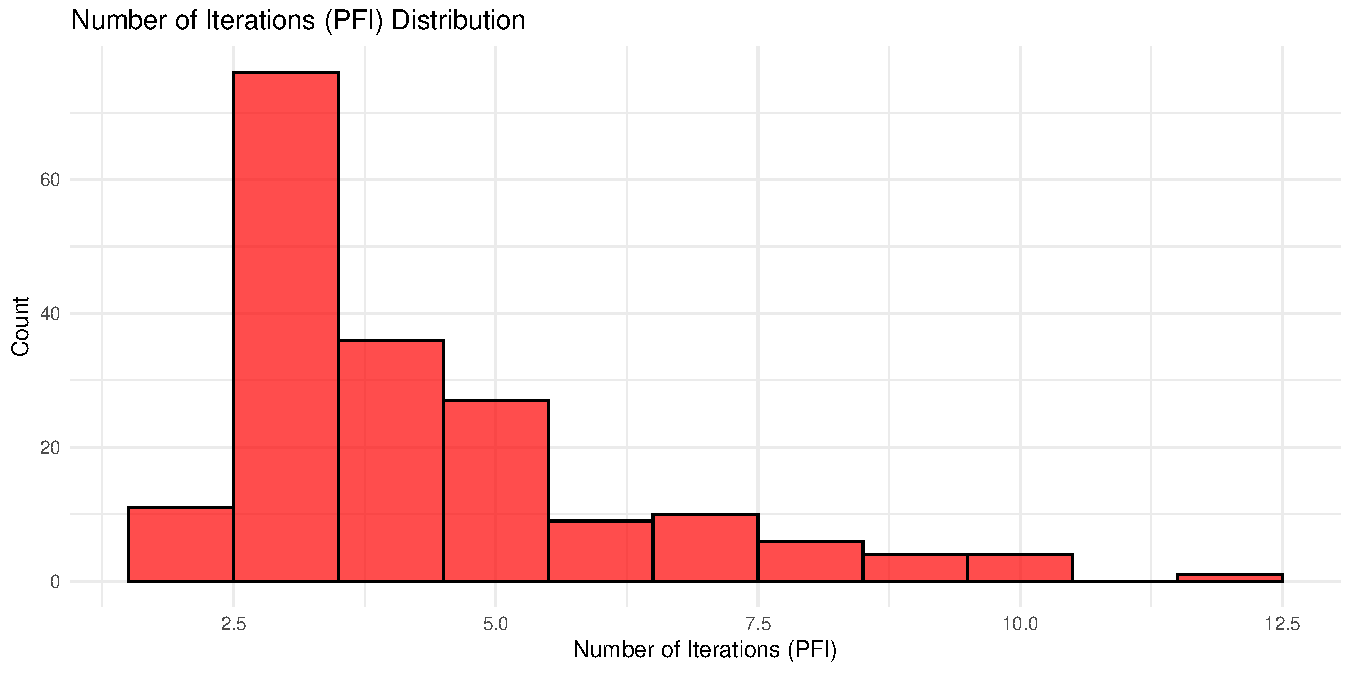
\includegraphics[width=\linewidth]{figures/num_iter_pfi_tpcds.pdf}
    \caption{Boxplot for number of iterations for PFI for TPCDS dataset}
    \label{fig:num_iter_pfi_tpcds}
\end{figure}


\subsubsection{TPC-H results}


%------------------------------------------------------------------------
\subsection{Results on randomly generated LPs}
We also test our solvers alongside Cplex, on packing LPs generated randomly.

We use a python script as a generator for packing linear programming (LP) problems.
It creates LP problem instances
based on the specified number of rules and variables.
For each rule, a random number of entries, ranging from 1 to
the total number of variables, is determined.
For every entry in a rule, a unique column number is randomly selected from
the available variables, ensuring that the same column is not used more than once for
the same rule. A random coefficient, between 0.1 and 1.0, is then assigned to
this column. The entire LP problem is represented as a space-separated string,
where the first entry denotes the number of rules, followed by the number of
entries for each rule, and then the column-coefficient pairs.
The main part of
the script generates a series of such LP problems, incrementally increasing the
number of rules and variables for each problem, and writes them to a text file.
This is how we get our randomly generated packing LPs with increasing sizes in the same format
as the query datasets.

We run our solvers, and also Cplex on this dataset, which provide us with numerical results
in the figures: \ref{fig:time_vs_size_random}, \ref{fig:lps_per_hour_random}, \ref{fig:size_time_random_large},
\ref{fig:speedup_cplex_less_1000.pdf}, and \ref{fig:speedup_cplex_random.pdf}.

We want to
explore those results to investigate how these solvers scale, and if the speedup
they provide is still substantial at larger LPs.


\begin{figure}[!htb]
    \centering
    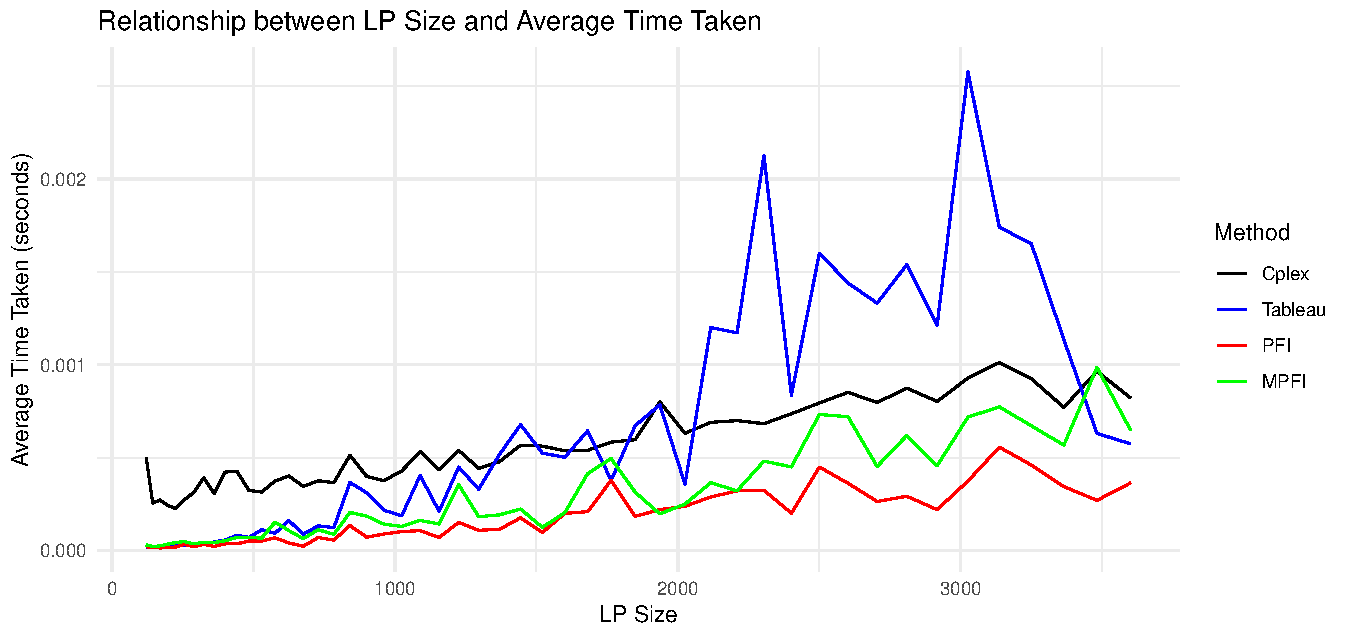
\includegraphics[width=0.8\textwidth]{figures/time_vs_size_random.pdf}
    \caption{Relation between LP size and time for the 3 simplex solvers and Cplex for randomly generated
        dataset with increasing LP size.}
    \label{fig:time_vs_size_random}
\end{figure}


\begin{table}[!htb]
    \centering
    \caption{Number of LPs Solved by Hour for the randomly generated dataset}
    \begin{tabular}{l|r}
        \toprule
        Method                     & Number of LPs \\
        \midrule
        Revised Simplex MPFU Umbra & 13,520,349    \\
        Tableau Simplex            & 6,963,530     \\
        Revised Simplex PFI        & 24,352,331    \\
        Cplex                      & 6,666,083     \\
        \bottomrule
    \end{tabular}
    \label{fig:lps_per_hour_random}
\end{table} 

We get the time profile in Figure \ref{fig:time_vs_size_random}.
We want to see the further evolution of this time profile, so we increase the number of generated LPs
and explore larger LPs, see Figure \ref{fig:size_time_random_large}.

\begin{figure}[!htb]
    \centering
    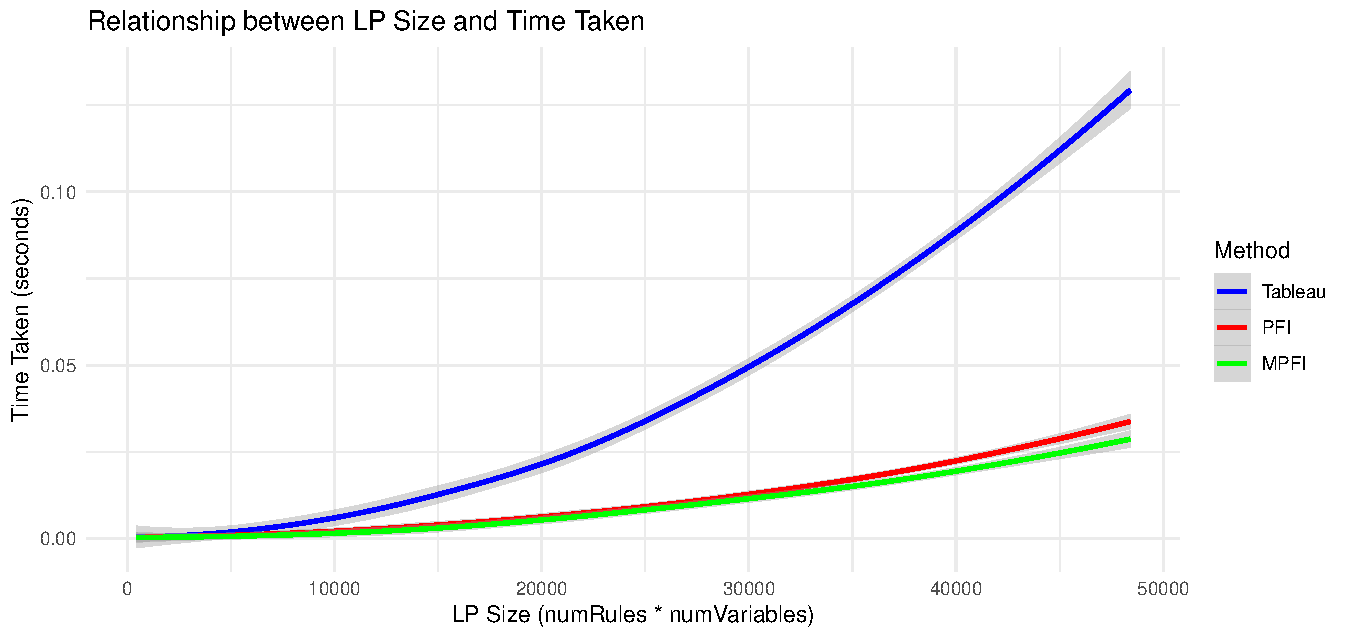
\includegraphics[width=\linewidth]{figures/size_time_random_large.pdf}
    \caption{Relation between LP size and time for the 3 simplex solvers for the randomly generated
        dataset with increasing LP size ranging up to 220 rules and 220 variables.}
    \label{fig:size_time_random_large}
\end{figure}

\begin{figure}[p]
    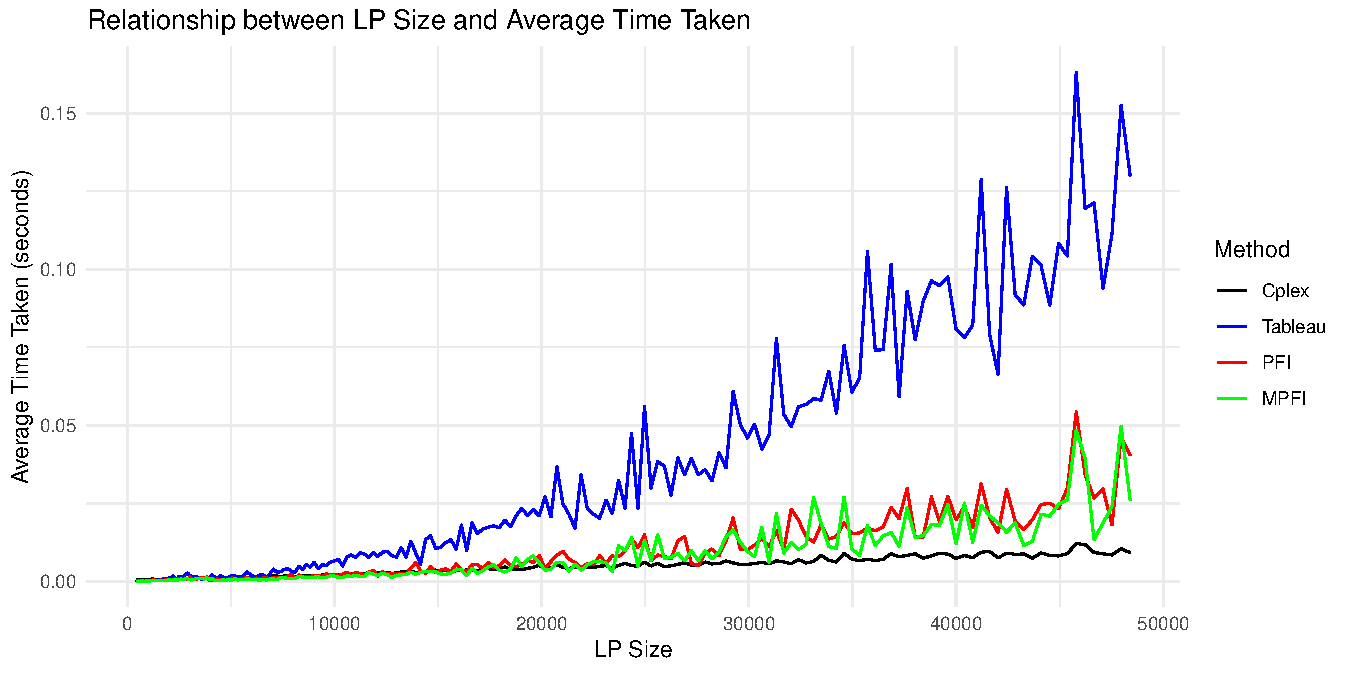
\includegraphics[width=0.8\paperwidth, height=\paperheight, keepaspectratio]{figures/cplex_vs_all_random_large.pdf}
    \caption{Relation between LP size and time for the 3 simplex solvers with CPLEX randomly generated
        dataset with increasing LP size ranging up to 220 rules and 220 variables.}
    \label{cplex_vs_all_random_large}
\end{figure}

\begin{figure}[!htb]
    \centering
    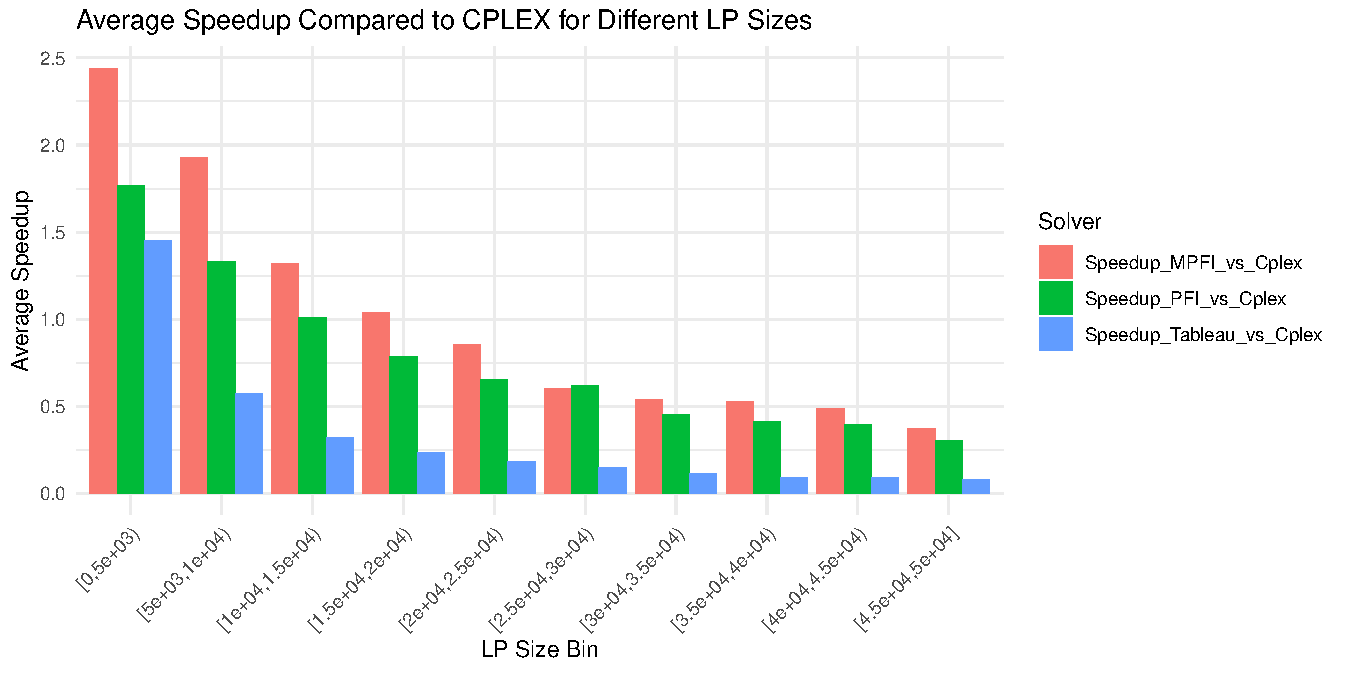
\includegraphics[width=\linewidth]{figures/speedup_vs_cplex_random_200.pdf}
    \caption{Speedup of the three solvers (how many times faster they are) compared to CPLEX for
        the randomly generated dataset for increasing LP size}
    \label{fig:speedup_cplex_random.pdf}
\end{figure}

\begin{figure}[!htb]
    \centering
    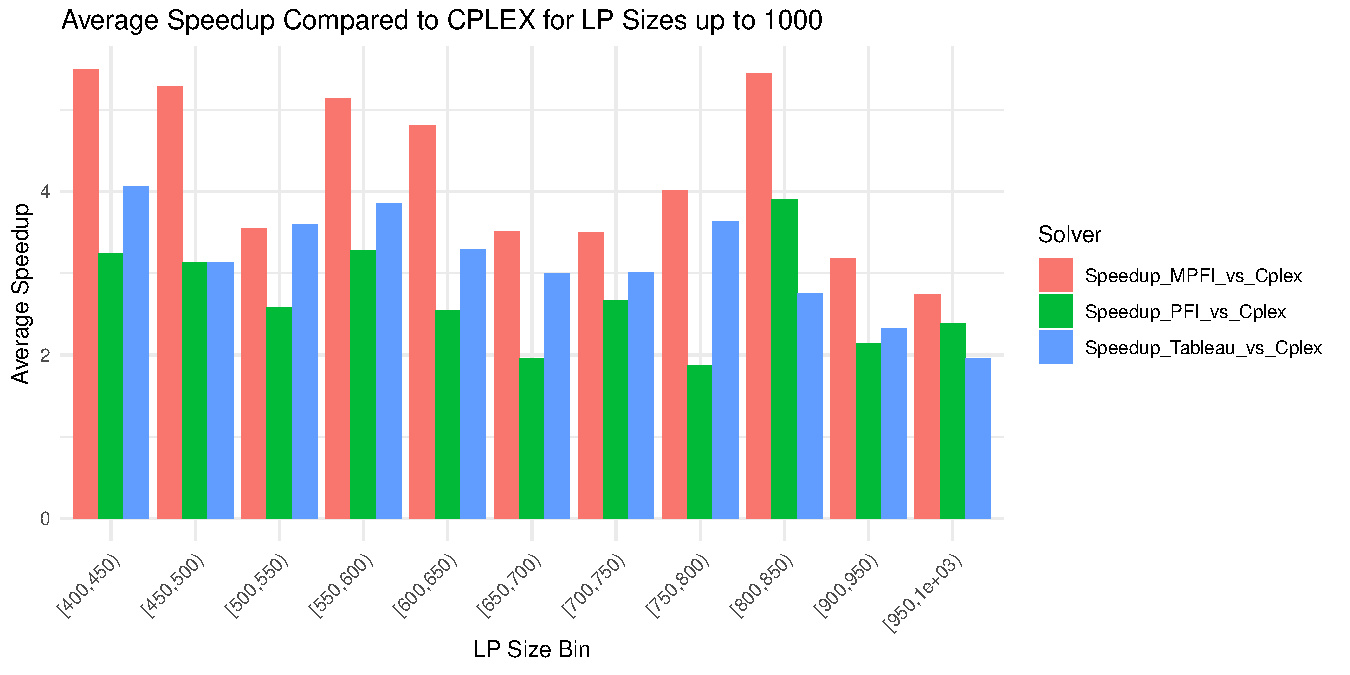
\includegraphics[width=\linewidth]{figures/speedup_cplex_less_1000.pdf}
    \caption{Speedup of the three solvers (how many times faster they are) compared to CPLEX for
        the randomly generated dataset for the LP size up to 1000}
    \label{fig:speedup_cplex_less_1000.pdf}
\end{figure}

%------------------------------------------------------------------------
%------------------------------------------------------------------------
\section{Analysis}
In the following section we will conduct an analysis of our various numerical results
and benchmarks.
We will discuss the
particularites of the structure of these LP problems, and if there are any
patterns in their solution
process. This analysis is based on observing the statistical results we obtained from
running different solvers on these problems. This will provide us with insight
regarding the optimization of these problems.

We will also analyse and compare the time performance for our implementation solvers,
Umbra's revised simplex with the Middle \gls{pfi} update variant, Cplex and HiGHS.


%------------------------------------------------------------------------
\subsection{Analysis JOB dataset}

\subsubsection{Structure and properties}
In  this subsection we will conduct an analysis the JOB dataset properties.

A opposed to what the linear programming research has dealt with, which is
very large problems, we are dealing with hundreds of small problems. The statistics
collected about the JOB dataset in the Table \ref{table_job_stats} prove this, since the LP size range is small, (number
of rules ranging from 1 to 19 and number of variables between 1 and 6).

Given the size of these LPs one might think the constraint matrices involved
are practically dense, however our results show differently. If we look at the densities
in the Table \ref{table_job_stats} we can see that the constraint matrix average density
for the JOB queries is around $0.6703$.

These matrices are represented
in the revised simplex algorithm by
sparse matrices but not as sparse as it would have been if the problem was large, i.e.
small matrices that are not small enough to be dense.

\subsubsection{Time efficiency}
From the table \ref{table_lps_hr_job}, we can see that the Tableau solver
outperforms the two other revised simplex solvers and Cplex. It records
the largest Query-Per-Hour metric, around $ 1.4 \texttt{billion}$ queries per hour.
The time profiles of the three solvers show that for the queries that have
an LP size less than 250 (we define the LP size as the product of the number 
of variables and the number of rules this LP has $\texttt{lp\_size} = m \times n$)
Tableau is the best out of the three. 
However, from $\texttt{lp\_size} \geq 250$ PFI outperforms the tableau method.
Meanwhile, the MPFI delivers the worst execution time out of the three solvers, for
this JOB dataset of small queries. 

Also, Cplex is slower than all other solvers for this dataset.

These results may be due to several reasons. We think most likely reason,
according to theoretical analysis of the functionalities of these solvers, and the documentation
of Cplex, is based on the small size of these LP problems.

\begin{itemize}
    \item Overhead of Cplex: Cplex, being a commercial solver, is designed to handle
    large-scale LPs. To do this, it incorporates many (in our case unnecessary) advanced techniques like 
    long initialization phases, presolving,
    where it attempts to simplify the LP, analyze it, identify special structures... While
    this can be highly beneficial for large and more complex problems, for small ones it 
    introduces unnecessary overhead.
    \item Simplicity of Tableau solver: our solver is very basic, skips unnecessary
    preprocessing or initialization. The bottleneck of the Tableau simplex solver
    is the Pivoting step, which includes row operations on dense matrices.
    For small problems, the data might fit entirely within the CPU cache, 
    making certain operations faster. The 1D dense matrix data structure may be a good 
    choice for this reason.
    \item Overhead of revised simplex methods: in the revised simplex method we start by
    preparing the sparse matrix format. This data structure offers a beneficial speedup 
    for larger sparser problems, but for small problems it represents an unnecessary 
    overhead, compared to the Tableau simplex, even though the latter uses a dense 
    representaion of the tableau, but in 1D vector, which may be more cache-friendly.
    The Revised Simplex method updates the matrix by enqueing an eta file to the pivots,
    but it still applies two basis multiplications BTRAN and FTRAN
    , which can be slower than the Pivoting operation of Tableau, especially for
     small problems.

\end{itemize}

It's worth noting that while the Tableau Simplex might be faster for some small LPs, 
it can be 
much slower than the Revised Simplex or CPLEX for larger or more complex problems. 
This is what we will discuss in  the next part of the analysis.

%------------------------------------------------------------------------
\subsection{Analysis of experiments on randomly generated LPs}
For small LP sizes, we observed that a basic implementation like tableau simplex
ouperform the revised simplex implementations as well as Cplex. However, for
larger LPs we come across other results. 
From figure \ref{fig:size_time_random_large} we see that Tableau does not scale well,
compared to revised simplex with PFI and MPFI update methods.

Also, starting from $\texttt{lp\_size} \geq 15,000$ approximately, we observe in Figure
\ref{cplex_vs_all_random_large} that Cplex starts outperforming our solvers.

\subsection{Why is highs so slow?}
using \texttt{linprog} from SciPy with HiGHS as a method can be 
slower than using the HiGHS interface directly, mainly due to the overhead, 
additional features and encapsulation.

